La obtención de la forma aparente de los Radios Característicos de los choques de Proa
no se obtiene de manera analítica de forma sencilla, por lo que recurrimos a hacer
aproximaciones a la forma de un choque dado, utilizando las cuádricas de revolución.
Éstas cuádricas dan un buen ajuste pero no son capaces de reproducir la forma completa
de un choque de proa dado, por lo que recurrimos al uso de dos cuádricas que en conjunto
ajustan a la forma completa del choque: una para la ``cabeza'' del choque, y otro para la cola.
Y cómo ya vimos en la sección , los radios característicos aparentes se pueden obtener de
manera sencilla para estas superficies.

\begin{figure*}
  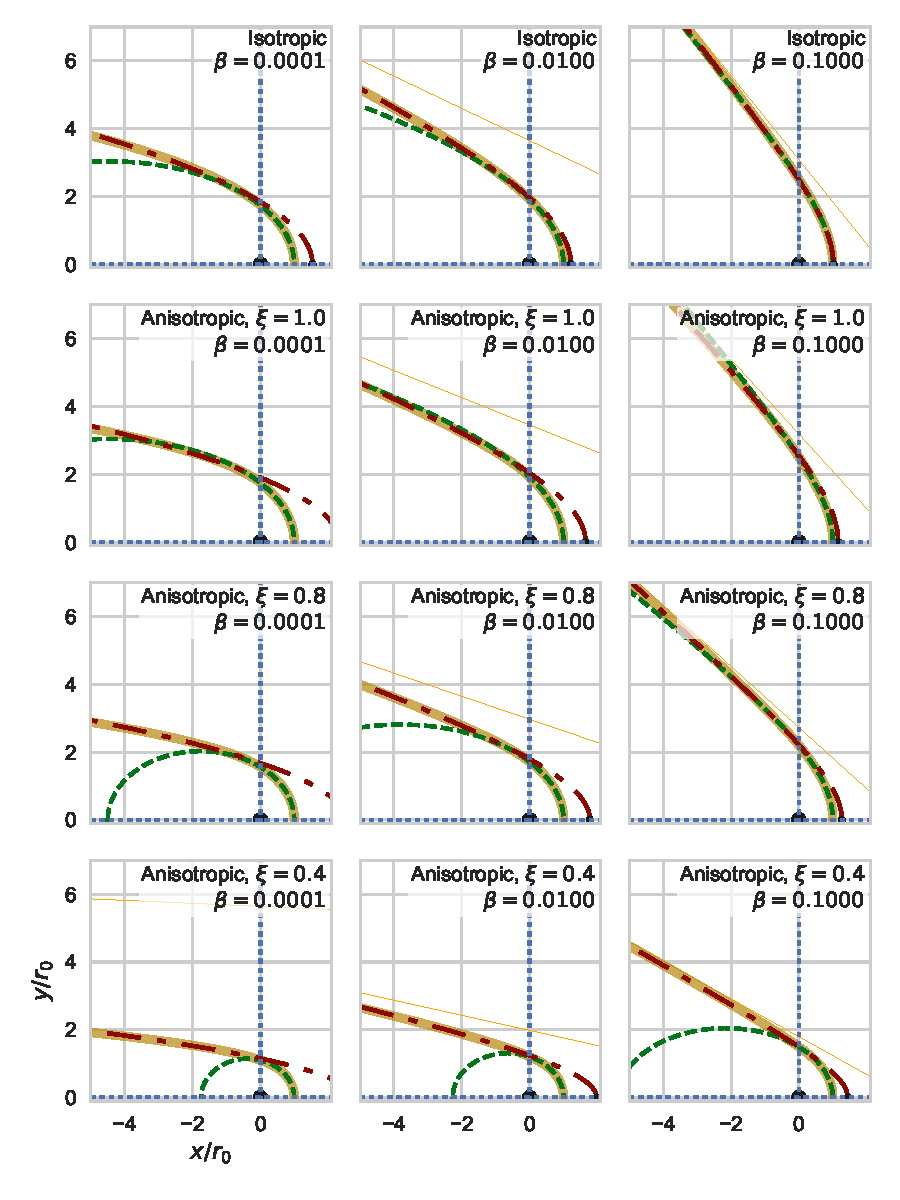
\includegraphics[width = 0.8\linewidth]{conic-head-tail-analytic}
  \label{fig:conic-head-tail-fit}
  \caption{Ajuste de dos cuádricas a las soluciones de capa delgada. La línea gruesa continua
    representa la forma de un choque bajo la aproximación de capa delgada (capítulo
    \ref{chap:hipersonica}) para los parámetros enlistados en cada pánel. La línea verde es el
    ajuste obtenido para la cabeza, mientras que la roja corresponde al ajuste para la cola.}
\end{figure*}


\section{Ajustes a la cabeza}

Utilizando las ecuación (\ref{eq:thc2})  de la sección \ref{sec:conic-char-radii} y las ecuaciones
(\ref{eq:CRW-Rc}) y (\ref{eq:CRW-R90}) de la sección \ref{sec:CRW-2-winds} podemos calcular el parámetro
$\theta_c$ que nos indicará el tipo de cónica que ajusta mejor a cada solución del modelo de capa delgada
en función de los parámetros
 $\beta$ y $\xi$:

 \begin{align}
   \tan\theta_c = \left|\frac{3\xi\left(1 + \beta^{1/2}\right)^2}{\left(1 - \xi\beta\right)^2
   \left(1 + \frac{1}{5}\xi\beta\right)} - \frac{2}{\left|1 - 2\gamma\right|}\right|^{1/2}
 \end{align}

 
 
\section{Ajustes a la cola}